%\documentclass[conference]{IEEEtran}
%\IEEEoverridecommandlockouts
%\documentclass[sigconf]{acmart}
%\let\Bbbk\relax %% fix bug
\documentclass[twocolumn,10pt]{article}
\usepackage[utf8]{inputenc}

% =======================
\usepackage{amssymb}
\usepackage{amsmath}
\usepackage{amstext}
\usepackage{amsopn}
%\usepackage{algorithmic}
\usepackage{graphicx}
\usepackage{textcomp}
\usepackage{xcolor}

\usepackage{textcomp}

\usepackage{boxedminipage}
\usepackage{enumerate}
\usepackage{multirow}
\usepackage{url}
\usepackage{times}
\usepackage{version}
% \usepackage[pdftex]{graphicx}
\usepackage{graphicx} 
\usepackage{epsfig}
\usepackage{epsf}
%\usepackage{graphics}
\usepackage{caption}
\usepackage{subfigure}
\usepackage{algorithm}
\usepackage{algpseudocode}
%\PassOptionsToPackage{bookmarks={false}}{hyperref}
%%%%%%%%%%%%
\usepackage{comment}
\usepackage{multicol}
\usepackage{booktabs}
\usepackage{dblfloatfix}
% ==========================
%\usepackage[a4paper, margin = 2.5cm]{geometry}

\AtBeginDocument{%
  \providecommand\BibTeX{{%
    \normalfont B\kern-0.5em{\scshape i\kern-0.25em b}\kern-0.8em\TeX}}}

\begin{document}

\title{The Accuracy of KNN, decision tree, random forest, SVM, neural network, naive Bayes classifier and PLA for early Prediction of Diabetes}

\author{Hsieh Cheng-Han}
\date{October 2022}
\maketitle

\section*{Abstract}
  This work compares the accuracy of some classifiers for early the prediction of diabetes. More specifically, 
  the research compares the accuracy of k-nearest neighbors (KNN) algorithm, decision tree, random forest, 
  support vector machine (SVM), neural network, naive Bayes classifier, and perceptron learning algorithm (PLA) on the prediction of diabetes, which 
  the dataset is collected with eight features, times of pregnancy, concentration of glucose in blood, blood 
  pressure, skin thickness,  concentration of insulin in blood, body mass index (BMI), the value of diabetes 
  pedigree function and age.

  The result show that XXX is the most accurate on the prediction of diabetes.

\section{Introduction}
\label{sec:Introduction}
  Diabetes is a chronic disease which may cause many complications. There're lots of reason that can put a person 
  at the highly risk of having diabetes, such as age, obesity, lack of exercies, and more on. So many reasons 
  interweave together making the manual prediction on diabetes is nearly impossible. However, lots of works \cite{MUJUMDAR2019292} \cite{MAHBOOBALAM2019100204} \cite{10.3389/fgene.2018.00515}
  show that it is possible to have high accuracy by using machine learning techniques, such as random forest, 
  K-means clustering, neural network, and so on. 

  By collecting the essential data of human body, prediction of diabetes can be turn into classification problem. 
  Imagine that an individual case with essential data is a point in hyperspace, if it is closer to the cluster
  having diabetes, this case is more likely to have diabetes in the future, otherwise, this case is more likely 
  healthy. But there are lots of machine learning techniques born to solve classification problem, it remains a 
  problem that which technique having the hightest accuracy on the prediction of diabetes. 

  To find out which techniques is more suitable to predict diabetes, this work examines the diagnosis of diabetes 
  using KNN algorithm, decision tree, random forest, SVM, neural network naive Bayes classifier, and PLA.
\section{Related works}
\label{sec:Related works}
  \bf{k-nearest neighbors (KNN) classification algorithm}: \rm{The} KNN classification algorithm is a supervised learning 
  method which is first developed by Fix and Hodges \cite{10.2307/1403797}. The idea of KNN is based on the idiom, 
  "birds of a feather flock together". By picking the $k$-nearest neighbors of a data point, the unkonwn class label 
  can be determined. Lots of works \cite{6528591} \cite{8276012} \cite{vijayan2014study} show the fact that KNN performs  
  well for prediction of diabetes disease.

  \bf{decision tree}: \rm{Unlike} KNN uses distance to determine the outcome, 
  decision tree uses a sequence of deicsion that maximize the information gain, which can distinguish the class label of 
  data as much as possible, to determine the outcome. Many works \cite{5893838} \cite{8342938} have applied deicsion tree 
  method and gain a good accuracy. The advantage of decision tree is fast, easy to implement, and the decision is clear. 
  But the disadvantage is that it is very likely over-fitting and the structure of tree will become more complex with the 
  more the class labels. To solve this problem, the following techniques is developed:

  \bf{random forst}: \rm{Instead} of a signle decision tree, random forest use lots of decision trees, which form a "forest". 
  The decision trees are constructed by random subset of dataset. The key differs random forest from decision tree is that 
  while decision trees consider all the possible feature splits, random forests only select a subset of those features, which 
  reduce the risk of overfitting, bias, and overall variance. In \cite{7972337} \cite{10.1007/978-981-16-2164-2_19}, random 
  forest shows that it can greatly reduce the problem of over-fitting of the single decision tree, and gain an ever higher accuracy.

  \bf{support vector machine (SVM)}: \rm{Given} a set of training datas, where each data is labeled as a binary class, such as $0$ and $1$, SVM training algorithm creates a model that assigns new examples to the binay labels by making it a non-probabilistic binary linear classifier. In addition, accroding to \cite{amari1999improving} \cite{hofmann2006support}, SVM can also use a method called kernel trick to effectively perform non-linear classification by implicitly mapping its inputs into a high-dimensional feature space.

  \bf{neural network}: 

  \bf{naive Bayes classifier}: 

  \bf{perceptron learning algorithm (PLA)}: 

\section{KNN}
  \rm{The} rough process of KNN algorithm is described as follow: suppose that there is a dataset which contain $N$ data point, denoted as 
  $(X_i,Y_i)$ where $X_i$ is the features of the i-th individuals data and $Y_i$ is the class label of it. Now 
  a data with unknown class label is given, denoted $(X, Y)$. By a preset distance function $d(P, Q)$, ordering the dataset 
  as $(X_{(1)}, Y_{(1)}), (X_{(2)}, Y_{(2)}), \cdots, (X_{(N)}, Y_{(N)})$ where $d(X_{(1)}, X)\leq d(X_{(2)}, X)\leq\cdots\leq d(X_{(N)}, X)$. 
  Pick the $k$-first class labels to determine the unknow class label, $Y$.

  The algorithm to find $k$ nearest neighbors is the soul of KNN algorithm. The naive way to do that is brute force. By calculating every 
  distance between the dataset and the undetermined data, the desired class can be easily obtained. The time complexity of brute force is $O(n)$. 
  Another way to find $k$ nearest neighbors is approximate nearest neighbors oh yeah (ANNOY). This approximate algorithm is used at Spotify 
  for music recommendations. 
  \begin{figure*}[htb]
    \centering
    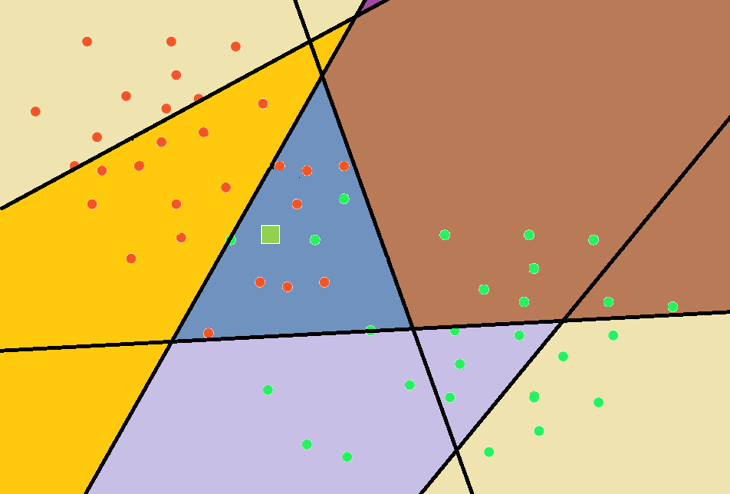
\includegraphics[scale=0.5]{assets/ANNOY-split.png}
    \caption{The region split by ANNOY.}
    \label{fig:ANNOY_split}
  \end{figure*}

  \begin{figure*}[htb]
    \centering
    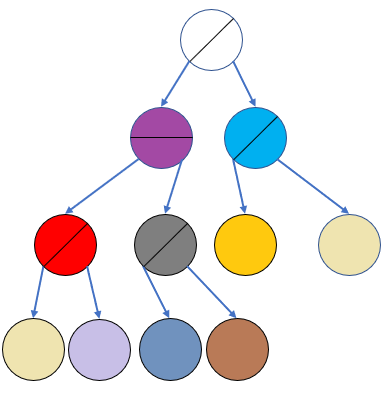
\includegraphics[scale=0.5]{assets/ANNOY-tree.png}
    \caption{The tree structure used by ANNOY.}
    \label{fig:ANNOY_tree}
  \end{figure*}
  Fig. \ref{fig:ANNOY_split} and Fig. \ref{fig:ANNOY_tree} give illustrations of how ANNOY works. The process of ANNOY is detailed as follow: In every iteration, two points are randomly chosen, denoted $\vec x_1,\vec x_2$, 
  and the hyperplane in the middle, whose equation is $\vec n^T\vec x=(\vec x_1-\vec x_2)^T\vec x=(\vec x_1-\vec x_2)^T(\vec x_1+\vec x_2)/2=b$ 
  separates all the points in dataset into two kind, "below" ($\vec n^T\vec x<b$) or "above" ($\vec n^T\vec x>b$). Also, in every iteration, a 
  binary tree structure is constructed whose left child contains all the points "below" the hyperplane and right child contains all the points "above". 
  The end condition is when a side of hyperplane contains points no more than $M$, which is a preset parameter. 
  When query a $k$ nearest neighbors of a point, recursively determine if the point "below" or "above" the hyperplane until reaching the leaf node. 
  The time complexity of construction is $O(n)$, and the time complexity of query is $O(\log n)$.
  But since the region searched may have less $k$ points, the search path shall cover both nodes if the point is too close to the hyperplane. This 
  techniques though may increase the search time, still, it can greatly increase the accuracy of searching.

\section{decision tree}
  Given a dataset, $D$, which contains $N$ data and class label, the construction of a decision tree can be described as 
  below: suppose there are $M$ candidate decisions, denoted $f_i$. A decision can separate dataset $D$ into $m$ kinds, denote 
  $D'_j$. The decision tree will adopt $\arg\max_{f} G(D, f)=I(D)-\sum^m_{j=1}\frac{N'_j}{N}I(D'_j)$ as node decision, 
  and then recursively construct the tree until the data in separated dataset have the same class label. 
  When a data with unknown class label comes, a decision tree determines recursively by the decision node until the leaf node.
  The function of calculating information, $I$, can be various from implementation. The most famous two information function is 
  entropy, and gini impurity. The formula of information entropy is $I_H(X)=-\sum_{x}p(x)\log_2p(x)$ 
  and gini impurity is $I_G(X)=1-\sum_{x}p(x)^2$.

\section{random forest}
  Given the fact that a signle decision tree can be easily over-fitting, a technique called "random forest" is developed. By 
  constructing $m$ decision trees with randomized subsets of training dataset, the different decision trees forms a "forest". 
  The process that random forest determine a data with unknown class label can be outlined as follow: suppose for a coming data, 
  $c_i$ decision trees in a random forest classify it as class $i$. Then the random forest will classify the data as class $\arg\max c_i$.

\section{SVM}
Given a dataset $D$ containing $N$ data points and a label with a binary class label of $0$ or $1$ representing the presence 
or absence of diabetes, respectively. Individually project each data point in the dataset $D$ onto the hyperplane, we can obtain 
a point $(X_{i1}, X_{i2}, ..., X_{ij}, ..., X_{in})$, where $X_{in}$ is the i-th individual data of $D$ and  j-th feature of $N$. 
After obtaining these points, these points are projected onto a hyperplane in $N+1$ dimensions to avoid situations where the 
data is non-linearly separable. 
In this case, using the kernel function below as the projection function for each data points in $D$ is a method of reducing 
the occurrence of non-linear separability: 
  $$\begin{bmatrix}x_1^{(2)} \\x_2^{(2)} \\... \\x_n^{(2)} \\ (\prod_{i=0}^{n} x_i)^{\frac{2}{n}} \end{bmatrix}$$
After this step, we can find a $N+1$ dimensions hyperplane $w$ that can separate the binary class labels of $0$ and $1$ for 
the data points. With this hyperplane trained on the training data, we can extend it to classify future data points that do 
not have binary class labels. 
In \cite{santhanam2015application}, we can use genetic algorithms to achieve finding better hyperplanes. The following are the 
steps to find the hyperplane using a genetic algorithm: Firstly, decide the level of generations ($l$), population size ($n$), 
variant ($v$), function constant ($b$), elite save rate ($p_e$), and mutations rate ($p_m$). Next, randomly select $N+1$ parameters 
of floating number between $0$ and $1$ in $w$, repeat it until $n$ hyperplanes are created. 
In the second step, use $w^t \cdot x - b$ \cite{kumari2013classification} to compare the binary labels of the training data. If 
$w^t \cdot x - b > 0$, the output is $1$; if $w^t \cdot x - b < 0$, the output is $0$. This determines the accuracy of the $n$ hyperplanes. 
Then, select the top $n \cdot p_e$ hyperplanes with high accuracy for crossover. The method is to take $v$ feature values from 
the parent chromosomes to replace or average (randomly) $v$ feature values from the mother chromosomes to create a new hyperplane. 
During the process, there is a probability of $p_m$ for random mutation of a feature value into a random floating number between 
$0$ and $1$. After mating $n-n \cdot p_e$ hyperplanes, return this step until the $l$th operation is completed and the best hyperplane 
is found.
 
\section{neural network}

\section{Naive Bayes classifier}

\section{PLA}

\section{Experiment result}

\section{Conclusion}

\bibliographystyle{IEEEtran}
\bibliography{main}
\end{document}

